% IE 643 project report (v2, after the primary-assessment review), course template.
\documentclass[twoside,english]{article}
\setlength{\oddsidemargin}{0.25 in}
\setlength{\evensidemargin}{-0.25 in}
\setlength{\topmargin}{-0.6 in}
\setlength{\textwidth}{6.5 in}
\setlength{\textheight}{8.5 in}
\setlength{\headsep}{0.75 in}
\setlength{\parindent}{0 in}
\setlength{\parskip}{0.07 in}
\setlength{\emergencystretch}{2em}

\usepackage{amsmath,amsfonts,graphicx,algorithm,caption}
\usepackage[noend]{algpseudocode}
\usepackage{hyperref}
\usepackage{natbib}
\usepackage[document]{ragged2e}
\usepackage{mathtools}
\usepackage{xcolor}
\usepackage{booktabs,array,enumitem}
\usepackage{tikz}
\usetikzlibrary{arrows.meta}
\usepackage{pgfplots}
\pgfplotsset{compat=1.17}
\graphicspath{{figures/}}

\newcounter{lecnum}
\renewcommand{\thepage}{\arabic{page}}
\renewcommand{\thesection}{\arabic{section}}
\renewcommand{\theequation}{\arabic{equation}}
\renewcommand{\thefigure}{\arabic{figure}}
\renewcommand{\thetable}{\arabic{table}}
\makeatletter
\def\BState{\State\hskip-\ALG@thistlm}
\makeatother

\newcommand{\lecture}[3]{
   \pagestyle{myheadings}
   \thispagestyle{plain}
   \newpage
   \setcounter{page}{1}
   \noindent
   \begin{center}
   \framebox{\vbox{\vspace{2mm}
    \hbox to 6.28in { {\bf IE 643: Deep Learning - Theory and Practice
        \hfill July-Dec 2026} }
    \vspace{4mm}
    \hbox to 6.28in { {\Large \parbox{6.0in}{\centering Project Report: #1}} }
    \vspace{2mm}
    \hbox to 6.28in { {\parbox{6.0in}{\centering\it Team Name: #2\\Team Members: #3}} }
    \vspace{2mm}}
   }
   \end{center}
   \vspace*{2mm}
}
\renewcommand{\cite}[1]{[#1]}
\def\beginrefs{\begin{list}{[\arabic{equation}]}{\usecounter{equation}
  \setlength{\leftmargin}{2.0truecm}\setlength{\labelsep}{0.4truecm}
  \setlength{\labelwidth}{1.6truecm}}}
\def\endrefs{\end{list}}
\def\bibentry#1{\item[\hbox{[#1]}]}

\begin{document}
\lecture{Vision-Language Model Guided Knowledge Distillation for Time-Series Anomaly Detection}
{[TEAM NAME -- replace before submission]}
{[MEMBERS AND ROLL NUMBERS -- replace before submission]}

\begin{abstract}
Anomalies in multivariate sensor data are rare, so detectors trained on few labels generalise poorly. We ask whether a frozen vision-language model (VLM) can supply knowledge that labels alone do not. Each window is rendered as a heatmap and a spectrogram and scored by frozen CLIP ViT-B/32 through \emph{learned prompts}: 7{,}168 context numbers trained through CLIP's frozen text encoder. The teacher's cross-fitted soft labels and image embeddings are distilled into a 95k-parameter convolutional bidirectional GRU that classifies and localises anomalies and runs about two orders of magnitude faster than the teacher. On four real-labelled datasets, with identical splits, identical initial weights, three seeds, five teachers, seven students and two classical baselines, prompt learning raises the teacher's test window AUPRC from 0.123 to 0.531 on Daphnet and from 0.037 to 0.989 on MetroPT-3, whose test set holds only two, visually obvious failures (a single-sensor rule chosen on training data already reaches 0.917, and the 95\% interval of the single-view teacher is 0.50--1.00). Distillation gives a consistent paired gain where labelled anomalies are scarcest. On MetroPT-3 (one training failure) the labels-only GRU memorises its single failure (train--test gap 0.40) and the distilled student raises point AUPRC from 0.524 to 0.889; when both models are regularized the gain is smaller but holds on every seed (+0.080 window, +0.061 point AUPRC, 3/3). On new, label-free series both deployed MetroPT students find 10 of 12 hidden real failures, and the distilled one has the higher point AUPRC (0.717 vs.\ 0.672) and event F1 (0.546 vs.\ 0.424). Where labels are plentiful or the task is easy (Credit Card, 3W) or the test subjects differ from training (Daphnet), distillation is neutral. An overfitting audit finds no memorisation on Credit Card and 3W, and a subject-shift gap of about 0.2 on Daphnet for every model, the teacher included. An independent re-computation reproduces every reported AUPRC exactly and re-scores the v1 models to their original values.
\end{abstract}

\section{Introduction and motivation}
An anomaly in a multivariate time series is a point, interval or pattern that departs from the behaviour expected in its operating context: a payment that does not fit the fraud-free population, a wearer's gait that freezes, a compressor whose pressure collapses before a failure. A useful detector must decide \emph{whether} a window is anomalous and \emph{where} the anomaly starts and ends, and it must do so cheaply enough to run next to the data source \cite{Pang21}.

Two facts motivate this project. First, anomaly labels are scarce, noisy and dataset-specific, so a detector trained only on them learns a narrow decision rule. Second, many anomalies are \emph{visual}: an engineer recognises a spike, a level shift or a burst of tremor at a glance on a plot. Large vision-language models (VLMs) \cite{Bordes24} such as CLIP were trained on hundreds of millions of image--text pairs, including charts and plots \cite{Radford21}, so their image encoders may carry a general prior for ``what an irregular signal looks like'' that complements the labels. VLMs are, however, far too large for edge deployment and were not trained on sensor data. Knowledge distillation \cite{Hinton15,Romero15} offers a way to transfer what such a model knows into a compact recurrent network that runs on the numeric signal directly.

We therefore ask three research questions, which also answer the central question raised at the primary assessment:
\begin{enumerate}[leftmargin=*,nosep]
\item[\textbf{RQ1}] Does a \emph{frozen} VLM, applied to rendered windows, provide an anomaly signal better than chance, and how should it be adapted without changing its weights?
\item[\textbf{RQ2}] Does distilling that signal into a GRU improve anomaly detection \emph{beyond training the same GRU on ground-truth labels alone}, on identical splits?
\item[\textbf{RQ3}] Which part of the teacher's knowledge matters (soft labels vs.\ embeddings), and how does it reach timestep localization?
\end{enumerate}

\section{Literature survey} \label{sec:litsurvey}
\textbf{Time-series anomaly detection.} Classical detectors score isolated observations or summary features; Isolation Forest isolates anomalies with random partitions and remains a strong unsupervised reference \cite{Liu08}. Deep methods model temporal context: LSTM forecasting with dynamic thresholds on spacecraft telemetry \cite{Hundman18}, stochastic recurrent reconstruction (OmniAnomaly) \cite{Su19}, adversarially trained auto-encoders (USAD) \cite{Audibert20} and attention-based association discrepancy (Anomaly Transformer) \cite{Xu22}. Pang et al.\ survey these families and stress that the anomaly definition and label availability determine which is appropriate \cite{Pang21}.

\textbf{Evaluation pitfalls.} Wu and Keogh show that several popular benchmarks contain trivial or mislabelled anomalies \cite{Wu21}, and Kim et al.\ show that the widely used point-adjusted F1 can make even random scores look strong \cite{Kim22}. We therefore report non-adjusted point metrics, event-level overlap metrics, and AUPRC together with the anomaly prevalence (the AUPRC of a random detector), and we tune every threshold on validation data.

\textbf{Time series as images and vision-language models.} Encoding a series as an image lets a vision model exploit spatial pattern priors: Gramian-angular and Markov-transition fields improved CNN classification \cite{Wang15}, and rendering irregular series as line plots let a pretrained vision transformer outperform specialised models \cite{Li23}. CLIP aligns an image encoder with a text encoder through contrastive pre-training and supports zero-shot classification by comparing an image with text prompts \cite{Radford21}. VLM4TS uses a pretrained vision encoder to screen plotted series and a large VLM to verify candidate intervals for zero-shot anomaly detection \cite{VLM4TS}. These works use the vision model at test time; none distils it into a small sequence model.

\textbf{Distillation and frozen-backbone adaptation.} Hinton et al.\ transfer a teacher's temperature-softened class distribution to a student \cite{Hinton15}; FitNets add intermediate-feature matching \cite{Romero15}, and contrastive representation distillation shows that matching representations carries more information than logits alone \cite{Tian20}. When a pretrained backbone must stay frozen, a linear probe on its features is the standard adaptation and is often more robust than fine-tuning \cite{Kumar22}. For vision-language models, CoOp \cite{Zhou22} keeps CLIP frozen and instead \emph{learns the words of the prompt}: a few continuous context vectors are optimised through the frozen text encoder, which consistently beats hand-written prompts in few-shot classification.

\textbf{Gap and position of this work.} We are not aware of prior work that (i) adapts a frozen CLIP encoder to sensor anomalies with learned prompts and a spectrogram view, (ii) distils both its soft labels and its image embedding into a recurrent student that runs on the raw numeric window, and (iii) evaluates, with matched ablations on four domains, whether this beats the same student trained on labels alone. The primary-assessment version of this project used zero-shot CLIP only and lacked the matched comparison; this report closes that gap.

\section{Response to the primary-assessment review} \label{sec:review}
\begin{table}[h]
\centering\small
\caption{Review points and where they are addressed.}
\label{tab:review}
\begin{tabular}{p{2.3in}p{3.9in}}
\toprule
Review point & Change in this revision \\
\midrule
Do teacher scores help beyond ground truth alone? & Paired GT-only vs.\ KD GRUs with identical splits and initial weights, 3 seeds, 4 datasets (Sec.~\ref{sec:results}, Table~\ref{tab:paired}). \\
Training objective unclear; which target trains which head & One implementation, Eq.~\eqref{eq:loss}, Table~\ref{tab:heads}, and a worked numeric example (Sec.~\ref{sec:objective}). \\
Low AUPRC on several datasets & Fixed the teacher's rendering, added a probe teacher, strengthened the student, AUPRC-based model selection, validation-tuned localization. \\
Compare frozen CLIP, GRU-GT and GRU-KD; AUPRC with prevalence; verify Air Quality labels; target one weak dataset & All models on the same test windows; prevalence in every table; Air Quality labels audited, found to be synthetic, dataset excluded (Sec.~\ref{sec:data}); Daphnet targeted with a step-by-step attribution (Table~\ref{tab:ladder}). \\
Literature review and motivation & Sections 1--2 rewritten. \\
Soft labels, localization, more experiments; novelty via comparisons and ablations & Learned-prompt and multi-view teachers, confidence-weighted KD, teacher-only and feature-KD ablations, window-gated localization, Isolation Forest and gradient-boosted-tree baselines, a label-free out-of-sample test, an overfitting audit, a regularized generalisation study and functional checks of each new component (Secs.~\ref{sec:gen}, \ref{sec:novelty}). \\
\bottomrule
\end{tabular}
\end{table}

\section{Proposed approach} \label{sec:our_proj}
\subsection{Work done before the primary-assessment review (v1)}
v1 rendered each standardised window as a heatmap using one global colour range fitted on training data, scored it with zero-shot CLIP against one normal and one anomalous prompt, and trained a two-layer unidirectional GRU with step BCE, window cross-entropy and a KL term on 1{,}000 teacher-scored windows. Its Daphnet controlled study (seed 42) gave frozen-CLIP test window AUPRC 0.029 (ROC-AUC 0.25, below chance) at prevalence 0.048, GRU-GT 0.280 and GRU-KD 0.394, with event F1 below 0.1.

\subsection{Work done after the review (v2)}
\textbf{Data and splits.} Each dataset is split once (Table~\ref{tab:data}); imputation and standardisation are fitted on training data only; windows never cross a recording, subject, instance or acquisition-block boundary. Every model in a dataset's comparison sees exactly the same windows.

\textbf{Teacher (RQ1), view 1.} Each standardised channel is clipped to $[-4,4]$ and drawn as one row of a $224\times224$ viridis heatmap (labels are never drawn). v1's global colour range spanned about $[-95,108]$ on Daphnet, so most windows became near-uniform images; on a Daphnet validation sample the clipped rendering raised probe AUPRC from 0.666 to 0.780 (line plots: 0.672). The frozen ViT-B/32 image encoder \cite{HFclip,GitCLIP} maps the image to a unit vector $e\in\mathbb{R}^{512}$. \textbf{View 2.} A spectrogram rendering stacks the short-time Fourier magnitude of each channel (Hann window, fixed log scale) channel$\times$frequency against time, because rhythmic anomalies (freezing-of-gait tremor at 3--8\,Hz, slugging, compressor cycling) are clearer in frequency than in amplitude.

\textbf{Teachers.} Every teacher uses the same frozen image encoder. (a) \emph{Zero-shot}: $e$ against the mean text embeddings of four normal and four anomalous hand-written prompts. (b) \emph{Linear probe}: logistic regression on $e$ (or on both views concatenated). (c) \emph{Learned prompts (CoOp, final teacher)}: the prompt ``[SOS] $v_1\dots v_{14}$ normal$\mid$anomalous . [EOS]'' has 14 learnable context vectors (7{,}168 numbers) initialised from the phrase \emph{``a heatmap of a multivariate sensor time series that looks''}; they pass through CLIP's frozen text encoder and are trained with cross-entropy on training windows, with $p(c\mid x)=\mathrm{softmax}_c(100\cos(e_x, f_{\mathrm{text}}(c)))$. With two views the class logits are averaged over the heatmap and spectrogram embeddings. A unit test confirms that the untrained learnable prompt reproduces CLIP's own text features exactly (maximum difference 0.0). \emph{Cross-fitting}: to keep a teacher from copying hard labels, its soft labels for training windows are out-of-fold. Windows are cut into blocks of 32, assigned round-robin to five folds, and each block is labelled by a teacher fitted on the other folds. (An initial version used five contiguous folds; it put MetroPT's single training failure inside one fold, so that fold's teacher had never seen a failure. The interleaved blocks fix this.) Up to 8{,}000 time-distributed training windows per dataset are scored.

\textbf{Student.} A Conv1d($F\!\to\!64$) + strided Conv1d($64\!\to\!64$, stride $d$) front-end learns local shape filters and shortens long windows ($d=4$ for Daphnet, 2 for 3W/MetroPT, 1 otherwise); a bidirectional GRU (64 units) gives per-step states $h_t$. A \emph{window head} maps mean+max pooled states $\bar h$ to two logits $z_w$; a \emph{step head} maps each $h_t$ to a logit, linearly upsampled back to length $L$; a training-only \emph{embedding head} $g(\bar h)\in\mathbb{R}^{512}$ is used for feature distillation. The deployed network has 94k--101k parameters, about 1/1500 of CLIP ViT-B/32 (151M).

\subsection{Training objective} \label{sec:objective}
\begin{equation}
\mathcal{L}=\underbrace{\mathrm{BCE}_{w}(z_s,y_{\mathrm{step}})}_{\text{step head, GT}}
+\beta\,\underbrace{\mathrm{CE}(z_w,y_{\mathrm{win}})}_{\text{window head, GT}}
+\lambda_{\mathrm{KD}}\,\underbrace{\tfrac{1}{n}\textstyle\sum_i w_i\,T^2\,\mathrm{KL}\!\left(p_{T,i}^{(T)}\,\Vert\,\mathrm{softmax}(z_{w,i}/T)\right)}_{\text{window head, teacher}}
+\lambda_{\mathrm{feat}}\,\underbrace{\left(1-\cos(g(\bar h),e)\right)}_{\text{embedding head, teacher}}
\label{eq:loss}
\end{equation}
with $p^{(T)}=\mathrm{softmax}(\log p/T)$, confidence weights $w_i=p_{T,i}(y_i)$ (the teacher's probability for the window's true class; $w_i=1$ without weighting), $T=2$, $\beta=1$, $\lambda_{\mathrm{KD}}=1$, $\lambda_{\mathrm{feat}}=0.5$, and step positive weight $w=\mathrm{clip}(\sqrt{n_{neg}/n_{pos}},1,25)$. The teacher terms are averaged only over teacher-scored windows; the validation loss never contains them.

\begin{table}[h]
\centering\small
\caption{Which target supervises which head, and the ablation variants.}
\label{tab:heads}
\begin{tabular}{lllll}
\toprule
Head & Output & Target & Loss & Weight \\
\midrule
Step & $z_s\in\mathbb{R}^L$ & ground-truth timestep labels & weighted BCE & 1 \\
Window & $z_w\in\mathbb{R}^2$ & ground-truth window label $\max_t y_t$ & CE & $\beta$ \\
Window & $z_w\in\mathbb{R}^2$ & teacher soft label $p_T$ (cross-fitted) & $w_i T^2$KL & $\lambda_{\mathrm{KD}}$ \\
Embedding & $g\in\mathbb{R}^{512}$ & frozen CLIP image embedding $e$ & $1-\cos$ & $\lambda_{\mathrm{feat}}$ \\
\midrule
\multicolumn{5}{p{6in}}{Variants: GRU-GT ($\lambda_{\mathrm{KD}}{=}\lambda_{\mathrm{feat}}{=}0$); KD-zero-shot; KD-probe ($\lambda_{\mathrm{feat}}{=}0$); KD-full (probe, all terms); teacher-only ($\beta{=}0$); KD-prompts (learned prompts, 2 views, $w_i{=}1$); \textbf{KD-prompts-conf} (learned prompts, 2 views, confidence-weighted; proposed).}\\
\bottomrule
\end{tabular}
\end{table}

\textbf{Worked example} ($T=2$). A window with $y_{\mathrm{win}}=1$ and $y_{\mathrm{step}}=[0,0,1,1]$ has teacher probabilities $p_T=[0.2,0.8]$, softened to $[0.333,0.667]$. If the student's window logits are $z_w=[0.1,0.9]$, then $\mathrm{softmax}(z_w)=[0.310,0.690]$ and $\mathrm{softmax}(z_w/2)=[0.401,0.599]$. The window CE is $-\log 0.690=0.371$; the KD term is $4\,(0.333\ln\tfrac{0.333}{0.401}+0.667\ln\tfrac{0.667}{0.599})=4\times0.0097=0.039$; the step BCE is averaged over the four steps with positives weighted by $w$; with confidence weighting the KD term is multiplied by $p_T(y{=}1)=0.8$, giving $0.031$; the feature term is $1-\cos(g,e)$. Teacher knowledge thus enters the window head (KD) and the shared encoder (feature term), which also feeds the step head.

\textbf{Optimisation.} AdamW (learning rate $2\cdot10^{-3}$, weight decay $10^{-4}$), batch 128, at most 20 epochs, gradient clipping 1.0, ReduceLROnPlateau, and early stopping with patience 5 on the \emph{validation AUPRC} (mean of window and step AUPRC), which tracks the reported metric better than the loss did in v1. For each seed, all variants start from the same initial weights.

\subsection{Localization}
Step scores from overlapping windows are averaged per timestep and then (i) gated by the window-head probability, $s_t\cdot \bar p_{w,t}^{\,\alpha}$ with $\alpha\in\{0,0.5,1\}$, which lets the teacher-informed window head suppress isolated step activations; (ii) smoothed with a centred moving average $k\in\{1,L/16,L/8,L/4\}$; (iii) thresholded at the value that maximises validation point-F1, or, when validation contains fewer than five anomalous events (only MetroPT, which has one), at the 99.9th percentile of normal validation scores (0.1\% false-alarm rate), because a threshold fitted to a single event proved unstable (0.004--0.35 across seeds); (iv) runs shorter than $m$ steps are removed, with $m$ maximising validation event-F1. $\alpha,k$ are chosen by validation point AUPRC. Teachers and window-only baselines spread each window score over its steps and use the same procedure without gating.

\section{Dataset details} \label{sec:data}
\begin{table}[h]
\centering\small
\caption{Datasets used in this revision (all with real labels). Prevalence is on the test split.}
\label{tab:data}
\begin{tabular}{p{0.9in}p{1.55in}p{1.6in}p{1.9in}}
\toprule
Dataset & Features / windows & Labels & Split \\
\midrule
Credit Card \cite{CreditCC} & 29 (V1--V28, Amount); $L{=}64$, stride 32 & fraud flag; test prevalence 0.074 (windows), 0.0013 (rows) & chronological 60/20/20 \\
Daphnet FoG \cite{Bachlin10,UCIdaphnet} & 9 accelerometer axes, 64\,Hz; $L{=}256$, stride 64 & freezing of gait; 0.048 / 0.022 & subject-disjoint: 7 train, S02 val, S04+S07 test \\
3W \cite{Vargas19,UCI3w} & 8 pressure/temperature/flow; 10\,s means; $L{=}120$, stride 30 & class$\neq$0 (incl.\ transients); 0.620 / 0.604 & instance-disjoint; 364 instances (real wells first, no hand-drawn) \\
MetroPT-3 \cite{Metro22,UCImetro} & 7 analog + 8 digital, 1\,min; $L{=}120$, stride 30 & 4 published failures; 0.062 / 0.063 & failure 1 train, 2 val, 3--4 test \\
\bottomrule
\end{tabular}
\end{table}

\textbf{Air Quality (excluded).} The review asked us to verify how the Air Quality labels were constructed. The UCI file has no anomaly labels: every positive was a synthetic event injected by the project (spikes, level shifts, drifts, noise bursts; in v1 each shifted all 12 sensors at once and the test split held only six events). Because such labels measure recovery of our own injected patterns rather than real anomalies, Air Quality is excluded from this benchmark. Its audited runs \cite{UCIair} (every injected event listed in \texttt{label\_audit.csv}) are kept separately for later inclusion.

\section{Experiments} \label{sec:exp}
For each dataset we evaluate, on identical test windows: five frozen-CLIP teachers (zero-shot; probe on view 1; probe on both views; learned prompts on view 1; learned prompts on both views), two established non-VLM detectors on window statistics (Isolation Forest \cite{Liu08}, unsupervised; histogram gradient-boosted trees \cite{Ke17}, supervised), and seven GRU students (Table~\ref{tab:heads}) with seeds 0, 1, 2 and identical initial weights per seed. To test generalisation, the labels-only GRU and the proposed student were also trained on every dataset with a \emph{regularized} recipe (weight EMA 0.99, gain/noise augmentation 0.15/0.05, learning rate $10^{-3}$, dropout 0.3, patience 6), with the same splits, teachers, seeds and initial weights. The configuration served by the interface is chosen per dataset and model by validation AUPRC only. The main ablation tables use the base configuration for every variant, so all variants remain directly comparable. Finally, an \emph{out-of-sample test} generates label-free series in each dataset's schema, either from normal held-out stretches (``bootstrap'') or from an AR(1) process fitted to normal training windows (``synthetic''). Hidden anomalies are injected: three real anomalies transplanted from the test split and one each of six generic shapes (spike, level shift, drift, noise burst, oscillation, stuck sensor). The models see only the CSV, and an answer key grades them afterwards. Metrics are window-, point- and event-level; AUPRC is reported with prevalence. All runs used a CPU (Ryzen 5 7535HS, 12 threads, PyTorch 2.15 CPU build \cite{Torch}; Transformers \cite{HFT}, scikit-learn \cite{Sklearn}, Matplotlib \cite{Mpl}); code: \texttt{scripts/run\_benchmark.py}, \texttt{scripts/finalize\_benchmark.py}.

\section{Results} \label{sec:results}
\textbf{Main comparison.} Table~\ref{tab:main} reports key models (all 14 are in \texttt{experiments/benchmark\_v2/RESULTS.md}); Fig.~\ref{fig:auprc} shows window AUPRC for every model against the prevalence line, the AUPRC of a random detector.

\begin{table}[h]
\centering\scriptsize
\caption{Held-out test results, base training configuration (students: mean $\pm$ std over seeds 0--2; regularized results in Table~\ref{tab:gen}). Prevalence: windows/timesteps.}
\label{tab:main}
\resizebox{\linewidth}{!}{\begin{tabular}{llccc}
\toprule
Dataset (test prev.) & Model & Window AUPRC & Point AUPRC & Event F1 \\
\midrule
Credit Card (0.074/0.001) & CLIP zero-shot (frozen) & 0.079 & 0.001 & 0.018 \\
 & CLIP linear probe (frozen backbone) & 0.217 & 0.006 & 0.000 \\
 & CLIP learned prompts, heatmap + spectrogram & 0.124 & 0.003 & 0.000 \\
 & Gradient-boosted trees & 0.767 & 0.024 & 0.622 \\
 & GRU, ground truth only & 0.823 $\pm$ 0.005 & 0.787 $\pm$ 0.010 & 0.799 $\pm$ 0.014 \\
 & GRU + KD (soft labels + CLIP features) & 0.808 $\pm$ 0.010 & 0.783 $\pm$ 0.006 & 0.805 $\pm$ 0.017 \\
 & GRU + KD (learned prompts, 2 views, confidence-weighted) & 0.801 $\pm$ 0.011 & 0.775 $\pm$ 0.004 & 0.792 $\pm$ 0.006 \\
\midrule
Daphnet FoG (0.048/0.022) & CLIP zero-shot (frozen) & 0.123 & 0.059 & 0.222 \\
 & CLIP linear probe (frozen backbone) & 0.542 & 0.404 & 0.351 \\
 & CLIP learned prompts, heatmap + spectrogram & 0.401 & 0.452 & 0.373 \\
 & Gradient-boosted trees & 0.350 & 0.211 & 0.246 \\
 & GRU, ground truth only & 0.627 $\pm$ 0.058 & 0.519 $\pm$ 0.062 & 0.345 $\pm$ 0.105 \\
 & GRU + KD (soft labels + CLIP features) & 0.640 $\pm$ 0.110 & 0.523 $\pm$ 0.062 & 0.319 $\pm$ 0.071 \\
 & GRU + KD (learned prompts, 2 views, confidence-weighted) & 0.592 $\pm$ 0.068 & 0.477 $\pm$ 0.031 & 0.252 $\pm$ 0.044 \\
\midrule
3W Oil (0.620/0.604) & CLIP zero-shot (frozen) & 0.771 & 0.769 & 0.745 \\
 & CLIP linear probe (frozen backbone) & 0.992 & 0.982 & 0.971 \\
 & CLIP learned prompts, heatmap + spectrogram & 0.971 & 0.960 & 0.912 \\
 & Gradient-boosted trees & 0.998 & 0.992 & 1.000 \\
 & GRU, ground truth only & 0.985 $\pm$ 0.003 & 0.978 $\pm$ 0.003 & 0.925 $\pm$ 0.039 \\
 & GRU + KD (soft labels + CLIP features) & 0.980 $\pm$ 0.004 & 0.976 $\pm$ 0.004 & 0.875 $\pm$ 0.109 \\
 & GRU + KD (learned prompts, 2 views, confidence-weighted) & 0.978 $\pm$ 0.004 & 0.978 $\pm$ 0.002 & 0.943 $\pm$ 0.009 \\
\midrule
MetroPT-3 (0.062/0.063) & CLIP zero-shot (frozen) & 0.037 & 0.039 & 0.000 \\
 & CLIP linear probe (frozen backbone) & 0.931 & 0.942 & 0.889 \\
 & CLIP learned prompts, heatmap + spectrogram & 0.998 & 0.999 & 0.857 \\
 & Gradient-boosted trees & 0.702 & 0.692 & 0.800 \\
 & GRU, ground truth only & 0.751 $\pm$ 0.137 & 0.524 $\pm$ 0.251 & 0.250 $\pm$ 0.433 \\
 & GRU + KD (soft labels + CLIP features) & 0.865 $\pm$ 0.021 & 0.870 $\pm$ 0.010 & 0.750 \\
 & GRU + KD (learned prompts, 2 views, confidence-weighted) & 0.876 $\pm$ 0.015 & 0.889 $\pm$ 0.006 & 0.722 $\pm$ 0.048 \\
\bottomrule
\end{tabular}}
\end{table}

\begin{figure}[h]
\centering
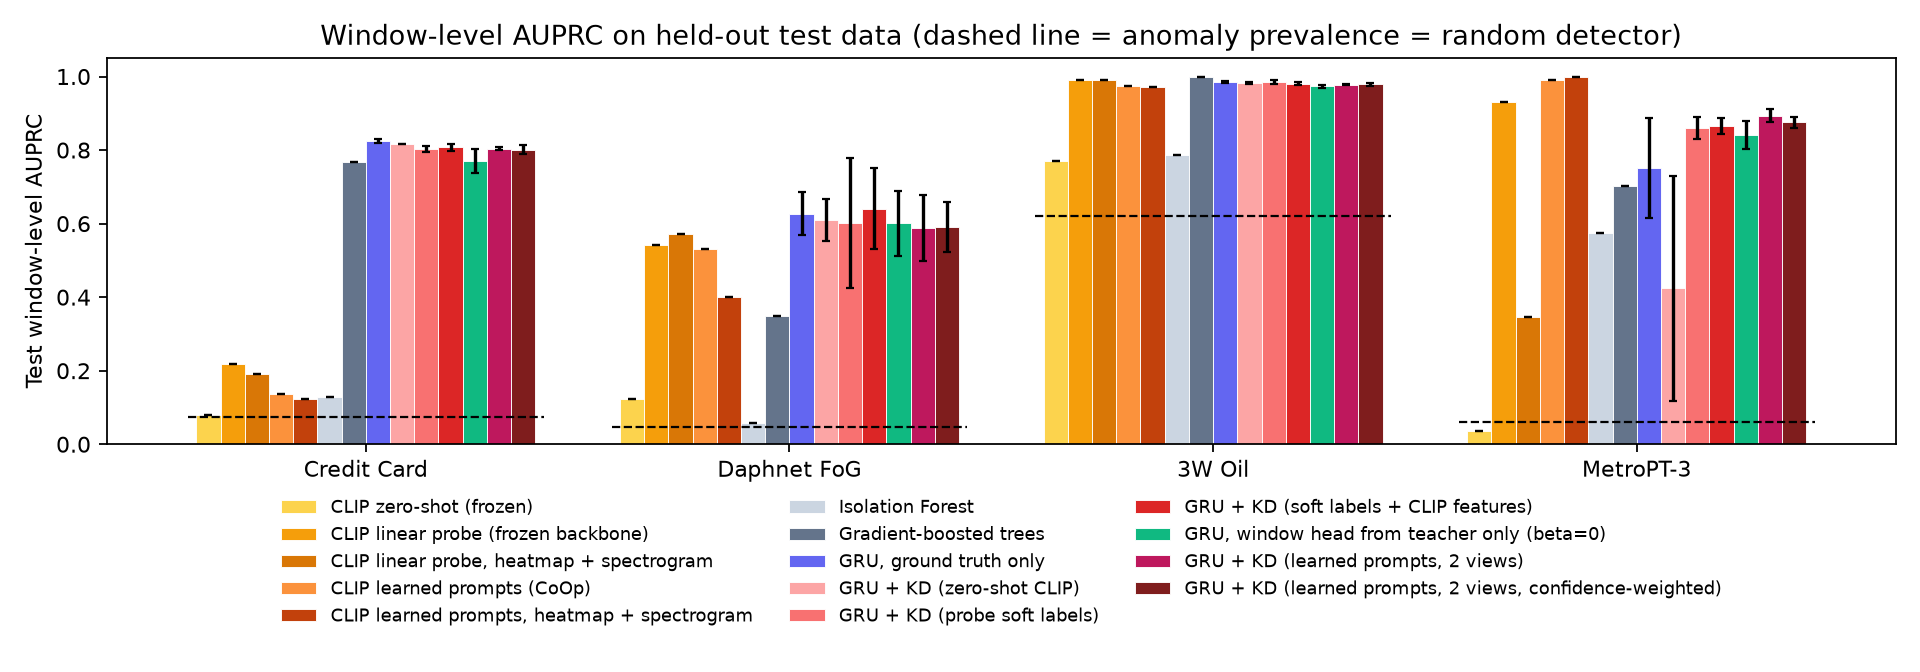
\includegraphics[width=\linewidth]{auprc_window.png}
\caption{Test window AUPRC of all teachers, baselines and students; dashed lines mark prevalence. Error bars: std over three seeds.}
\label{fig:auprc}
\end{figure}

\textbf{RQ1: the frozen VLM teacher.} Zero-shot CLIP is near random on every dataset (MetroPT 0.037 at prevalence 0.062). Adapting it without touching its weights changes this completely. Learned prompts reach window AUPRC 0.989 on MetroPT (0.998 with the spectrogram view), 0.974 on 3W and 0.531 on Daphnet. The linear probe is a strong alternative (0.931, 0.992, 0.542). The spectrogram view helps MetroPT but lowers Daphnet's window ranking (0.401), so view choice is dataset-dependent. On Credit Card every teacher is weak (best 0.217): a heatmap of 64 independent transactions carries little visual structure.

\textbf{Is MetroPT's 0.989 too good?} We audited it (\texttt{metropt/AUDIT.md}).
\begin{itemize}[leftmargin=*,nosep]
\item \emph{No leakage.} Training, validation and test share no sequence, and their failures are different events (1, 2 and 3+4). No test failure window is a near-duplicate of a training window: test failures lie further from the training failure than from training normal data (median per-value distance 0.51 vs.\ 0.42).
\item \emph{An easy test.} The window mean of a single sensor, DV\_pressure (sensor and sign chosen on training data, where it ranks first at 0.239), reaches \textbf{0.917} test AUPRC. The test failures are louder than the subtle training failure.
\item \emph{One event dominates.} Failure~3 lasts about two days and supplies most anomalous windows. Per event, the single-view learned prompts score 1.000 on failure~3 but 0.498 on failure~4; the two-view teacher scores 0.998 and 1.000.
\item \emph{Wide uncertainty.} A block bootstrap over test events and normal blocks gives 95\% intervals of 0.50--1.00 (learned prompts) and 0.09--1.00 (probe).
\end{itemize}
The high score is therefore genuine but rests on two events. It shows that the teacher generalises from one subtle failure to two obvious ones, not that it is a near-perfect detector. The one-sensor rule also outperforms every trained student on this test set; we report it as an additional reference.

\textbf{RQ2: does distillation beat labels alone?} Table~\ref{tab:paired} gives paired differences against the same GRU trained on labels only.

\begin{table}[h]
\centering\small
\caption{Paired change vs.\ the labels-only GRU (same split, same initial weights, base training; regularized in Table~\ref{tab:pairedreg}), mean over seeds and number of seeds improved, for the proposed student (KD with learned prompts, two views, confidence-weighted) and the probe-based full KD.}
\label{tab:paired}
\begin{tabular}{lcccccc}
\toprule
 & \multicolumn{3}{c}{Proposed (learned prompts)} & \multicolumn{3}{c}{Probe + features} \\
Dataset & $\Delta$ window AP & $\Delta$ point AP & $\Delta$ event F1 & $\Delta$ window AP & $\Delta$ point AP & $\Delta$ event F1 \\
\midrule
MetroPT-3 & +0.124 (3/3) & +0.365 (3/3) & +0.472 (2/3) & +0.114 (2/3) & +0.345 (3/3) & +0.500 (2/3) \\
Daphnet FoG & $-$0.035 (0/3) & $-$0.042 (1/3) & $-$0.093 (1/3) & +0.013 (2/3) & +0.004 (2/3) & $-$0.026 (2/3) \\
3W Oil & $-$0.007 (0/3) & +0.001 (1/3) & +0.018 (1/3) & $-$0.005 (1/3) & $-$0.002 (1/3) & $-$0.050 (1/3) \\
Credit Card & $-$0.022 (0/3) & $-$0.012 (1/3) & $-$0.007 (1/3) & $-$0.016 (0/3) & $-$0.004 (1/3) & +0.006 (2/3) \\
\bottomrule
\end{tabular}
\end{table}

The answer depends on how much labelled anomaly the student sees. MetroPT's training split contains a single failure; the labels-only GRU is unstable across seeds (point AUPRC $0.524\pm0.251$) and the distilled student is both better and stable ($0.889\pm0.006$; event F1 0.250 $\rightarrow$ 0.722). Both still trail the training-chosen one-sensor rule (window AUPRC 0.917 vs.\ 0.876 for the student). Part of this gain, however, reflects an overfitting baseline: the labels-only GRU scores 1.000 on training data and its train--test gap is 0.40 (Sec.~\ref{sec:gen}). When both models are regularized, the labels-only GRU rises to 0.821 point AUPRC and the gain shrinks to +0.061 point and +0.080 window AUPRC, still on all three seeds, with event F1 +0.242 (2/3 seeds; Table~\ref{tab:pairedreg}). We claim this smaller, regularized gain as the effect of distillation: the teacher supplies generalisation that one training failure cannot teach, judged on only two test failures. On 3W (prevalence 0.62, all models $\geq$0.97) and Credit Card (rows are independent transactions) the teacher adds nothing measurable. On Daphnet the test subjects differ from the training subjects. The probe-based KD is marginally better than labels alone ($0.640$ vs.\ $0.627$), but the learned-prompt student is slightly worse; with seed std of 0.06--0.11 neither difference is significant.

\textbf{RQ3: which knowledge matters.} On MetroPT, soft labels alone already give most of the gain (KD-probe point AUPRC 0.858). Adding CLIP features (0.870) and learned two-view prompts (0.889--0.890) adds a little more, and even a window head trained \emph{only} on teacher labels ($\beta=0$) reaches 0.828. Confidence weighting did not help on average: it is within one std of unweighted KD on every dataset. Zero-shot soft labels help MetroPT's point AUPRC but hurt its window AUPRC ($0.424\pm0.306$), so an unadapted teacher is a risk.

\textbf{Targeted dataset: why Daphnet's score rose.} Table~\ref{tab:ladder} re-scores the v1 models on the identical test split (subjects S04, S07; window prevalence 0.048) and adds one change at a time (Fig.~\ref{fig:daphnet}). The v1 numbers are reproduced exactly (0.056 point AUPRC for the v1 app checkpoint, 0.280/0.394 window AUPRC for the v1 controlled study), which shows the evaluation is unchanged in scale. Every AUPRC was also recomputed directly with scikit-learn from the saved predictions, with zero difference. Multiplying scores by 100 leaves AUPRC unchanged, and random scores or shuffled labels fall to the prevalence (\texttt{VERIFICATION.md}).

\begin{table}[h]
\centering\small
\caption{Daphnet attribution on the identical test split (window prevalence 0.048, point 0.022).}
\label{tab:ladder}
\begin{tabular}{lcc}
\toprule
Model & Window AUPRC & Point AUPRC \\
\midrule
v1 teacher: zero-shot CLIP, global-range heatmap, 2 prompts & 0.029 & -- \\
v2 teacher: zero-shot CLIP, clipped heatmap, 8 prompts & 0.123 & 0.059 \\
v2 teacher: learned prompts (CoOp), heatmap & 0.531 & 0.471 \\
v1 app checkpoint (50 teacher windows) & 0.058 & 0.056 \\
v1 controlled study, GRU + zero-shot KD, v1 scoring & 0.394 & 0.307 \\
\quad + v2 validation-tuned localization & 0.394 & 0.377 \\
v2 GRU (conv front-end, BiGRU, AUPRC selection), labels only, 3 seeds & 0.627 & 0.519 \\
v2 GRU + KD (probe + CLIP features), 3 seeds & 0.640 & 0.523 \\
v2 GRU, labels only, regularized training, 3 seeds & 0.659 & 0.535 \\
v2 GRU + KD (learned prompts), regularized training, 3 seeds & 0.655 & 0.549 \\
\bottomrule
\end{tabular}
\end{table}

\begin{figure}[h]
\centering
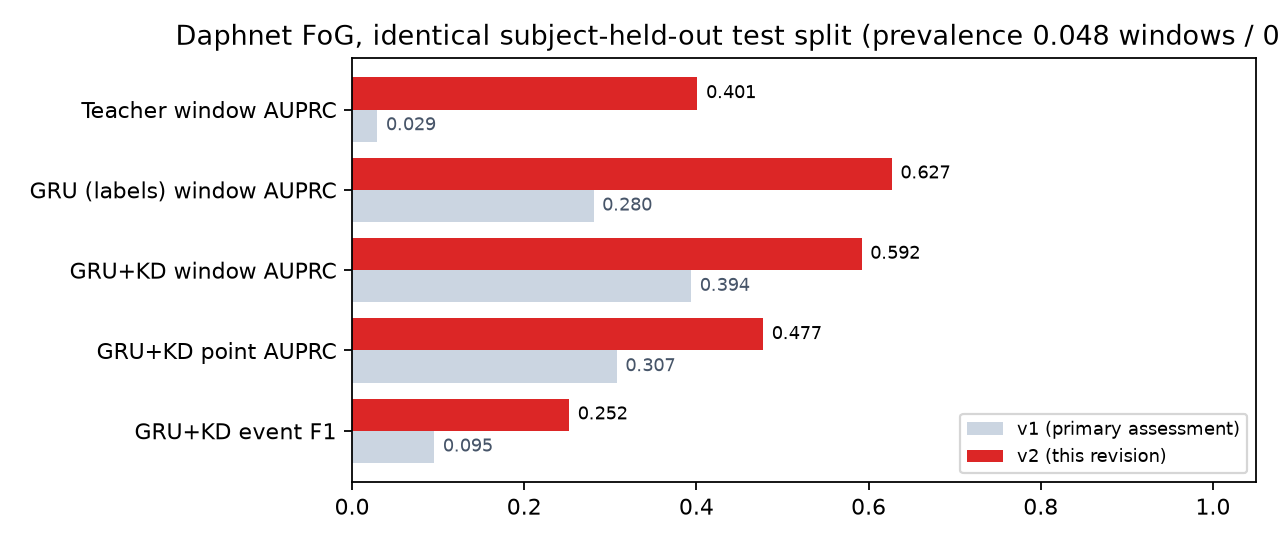
\includegraphics[width=0.75\linewidth]{daphnet_before_after.png}
\caption{Daphnet, v1 (primary assessment) vs.\ this revision on the identical test split. The v2 teacher shown is the two-view learned-prompt teacher; the single-view teacher reaches 0.531.}
\label{fig:daphnet}
\end{figure}

\textbf{Out-of-sample test.} Each dataset receives 2 backgrounds $\times$ 2 seeds of label-free generated series with 9 hidden anomalies each, scored by the deployed checkpoints (\texttt{OUT\_OF\_SAMPLE.md}).
\begin{itemize}[leftmargin=*,nosep]
\item \emph{MetroPT.} Both students find 10/12 hidden real failures (Fig.~\ref{fig:oos}). The distilled student has the higher point AUPRC (0.717 vs.\ 0.672) and event F1 (0.546 vs.\ 0.424), partly because it also flags 4 of 24 generic anomalies against none for the labels-only GRU. With the base (unregularized) checkpoints the result was 10/12 vs.\ 0/12; that difference came from the overfitted labels-only GRU, so we do not claim it.
\item \emph{Other datasets.} Students find 3--6 of 6 real anomalies per background, and the student and the labels-only GRU perform similarly.
\item \emph{Generic shapes.} Spikes, stuck sensors and shifts are mostly missed. The detectors are specialists for the anomaly class they were trained on, which is the main limitation found.
\item \emph{Synthetic backgrounds.} On the fully synthetic AR(1) background the teacher flags nothing (Credit Card, Daphnet) or, on 3W, every model flags almost the whole series. That background is too unlike the real signals to be informative except on MetroPT.
\end{itemize}

\begin{figure}[h]
\centering
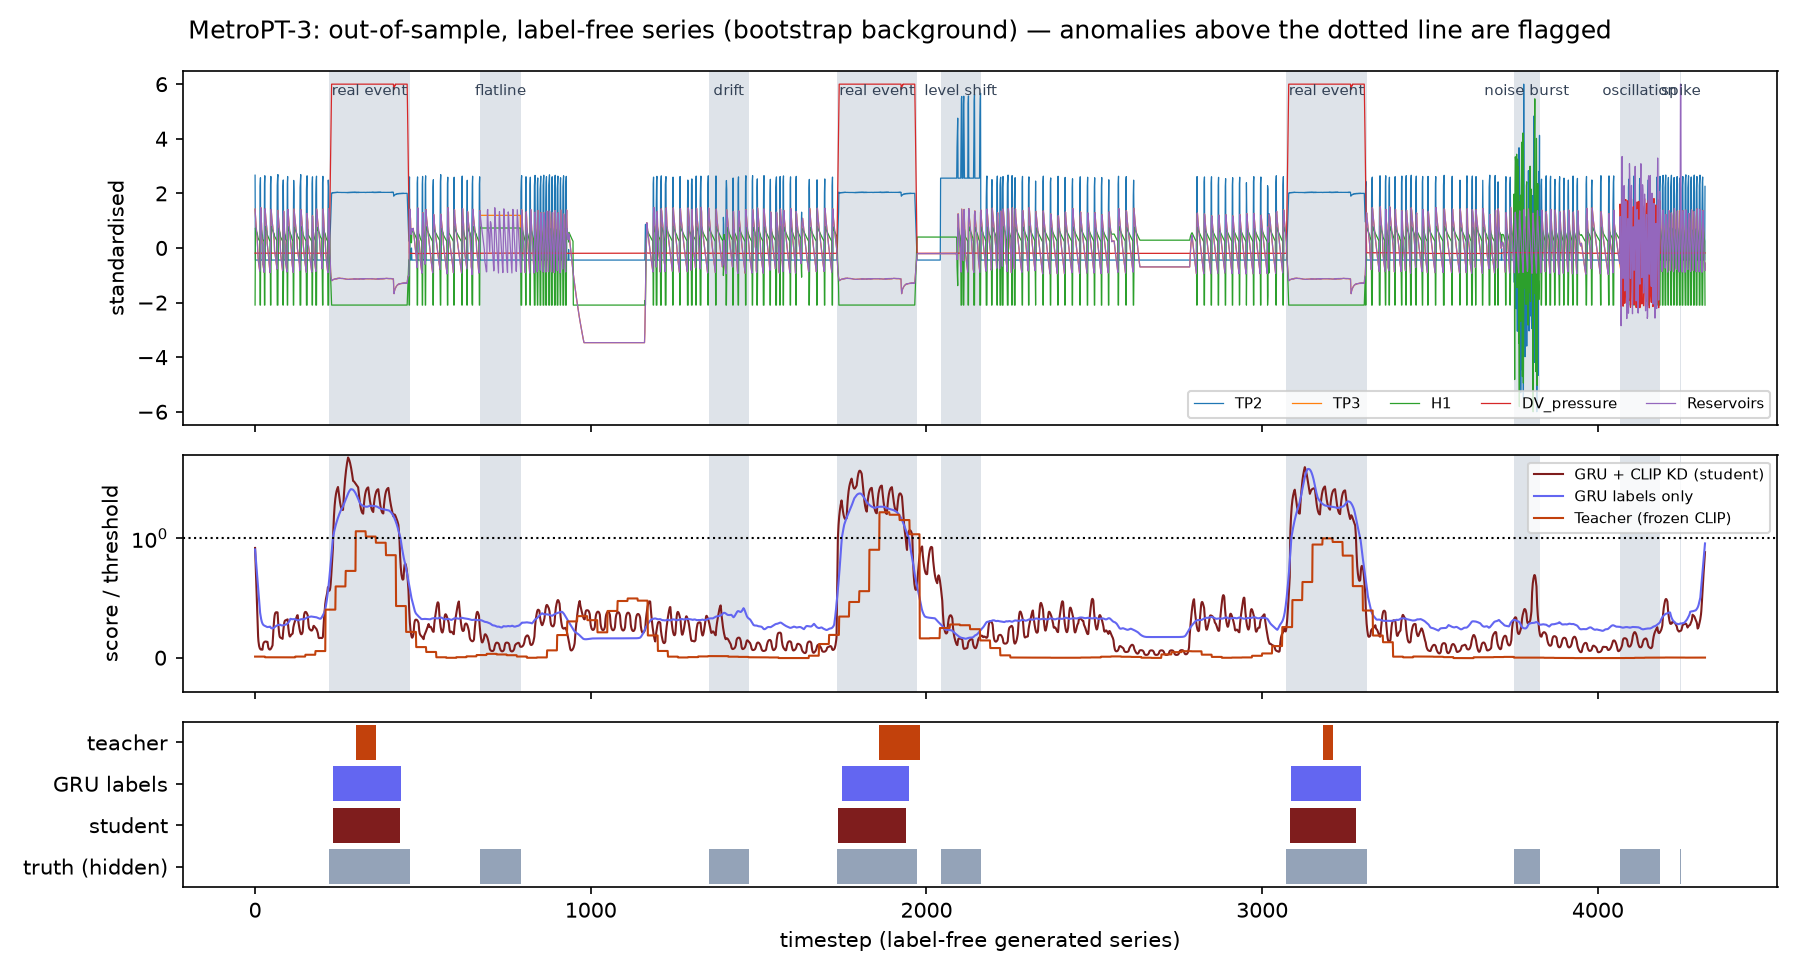
\includegraphics[width=\linewidth]{oos_metropt_bootstrap.png}
\caption{Label-free MetroPT series built from held-out normal data with nine hidden anomalies (grey; type above). Scores are divided by each model's validation threshold (dotted line). With the deployed models all three detectors flag the three transplanted real failures and miss the generic shapes. With the base checkpoints the labels-only GRU flagged none of the real failures (\texttt{oos\_metropt\_bootstrap\_base\_checkpoints.png}).}
\label{fig:oos}
\end{figure}

\section{Overfitting and generalisation} \label{sec:gen}
\textbf{Overfitting audit.} Table~\ref{tab:overfit} compares window AUPRC on the training, validation and test splits of the deployed checkpoints; teacher training scores are out-of-fold, as used for distillation (\texttt{OVERFITTING.md}).
\begin{itemize}[leftmargin=*,nosep]
\item \emph{Credit Card and 3W:} no overfitting; train and test scores agree within 0.04.
\item \emph{Daphnet:} a gap of about 0.2 for every model, including the teacher, whose training scores are out-of-fold and so cannot be memorised. The gap therefore comes from testing on different people (subject shift), not from memorisation.
\item \emph{MetroPT:} the base labels-only GRU scored 1.000 on train and 0.597 on test for its best seed (gap 0.40), i.e.\ it memorised its single training failure. Distillation reduced the gap to 0.11, and regularization to 0.14 (labels only) and 0.10 (distilled). The teachers' test scores exceed their out-of-fold training scores because the test failures are louder than the training failure.
\item \emph{Training dynamics:} the best validation epoch is 1--3 on Credit Card, Daphnet and MetroPT, and validation AUPRC falls by up to 0.14 afterwards, so early stopping on validation AUPRC is essential.
\end{itemize}

\begin{table}[h]
\centering\small
\caption{Overfitting audit: window AUPRC per split for the deployed checkpoints (best validation seed). Teacher train scores are out-of-fold.}
\label{tab:overfit}
\begin{tabular}{llcccc}
\toprule
Dataset (prev.\ train/val/test) & Model & Train & Val & Test & Train $-$ test \\
\midrule
Credit Card (0.098/0.058/0.074) & GRU, labels only & 0.792 & 0.802 & 0.826 & $-$0.034 \\
 & GRU + KD (proposed) & 0.806 & 0.785 & 0.791 & +0.015 \\
 & Teacher: learned prompts, 2 views & 0.321 & 0.086 & 0.124 & +0.197 \\
\midrule
Daphnet (0.171/0.189/0.048) & GRU, labels only & 0.862 & 0.842 & 0.641 & +0.221 \\
 & GRU + KD (proposed) & 0.828 & 0.843 & 0.634 & +0.195 \\
 & Teacher: learned prompts, 2 views & 0.645 & 0.665 & 0.401 & +0.244 \\
\midrule
3W (0.654/0.704/0.620) & GRU, labels only & 0.987 & 0.993 & 0.987 & $-$0.000 \\
 & GRU + KD (proposed) & 0.982 & 0.989 & 0.983 & $-$0.001 \\
 & Teacher: learned prompts, 2 views & 0.940 & 0.976 & 0.971 & $-$0.031 \\
\midrule
MetroPT-3 (0.007/0.009/0.062) & GRU, labels only & 1.000 & 1.000 & 0.856 & +0.144 \\
 & GRU + KD (proposed) & 1.000 & 1.000 & 0.899 & +0.101 \\
 & Teacher: learned prompts, 2 views & 0.842 & 0.894 & 0.998 & $-$0.156 \\
\bottomrule
\end{tabular}
\end{table}

\textbf{Generalisation study.} Table~\ref{tab:gen} compares the base and the regularized recipe for the labels-only GRU and the proposed student (\texttt{GENERALISATION.md}). Regularization lowers the seed variance and the train--test gap exactly where the base models overfit: on Daphnet the distilled student's window AUPRC rises from 0.592 to 0.655 and its seed std halves (0.068 $\rightarrow$ 0.030); on MetroPT the labels-only GRU's gap falls from 0.40 to 0.14 and its point AUPRC rises from 0.524 to 0.821. Credit Card and 3W are unchanged. Validation, however, separates the two recipes only weakly: MetroPT's validation split holds a single failure and saturates at 1.000 for both, and on Daphnet and 3W the differences are below 0.005. The deployed choice is therefore a near-tie under a pre-set rule, and we present regularization as a robustness improvement rather than a validated win. (Averaged over all five Daphnet student variants, the base recipe had the higher validation AUPRC, 0.834 vs.\ 0.830, which is why it is used for the ablation tables.)

\begin{table}[h]
\centering\small
\caption{Base vs.\ regularized training (mean over seeds 0--2). Selected: the recipe with the higher mean validation AUPRC; deployed in the interface.}
\label{tab:gen}
\resizebox{\linewidth}{!}{%
\begin{tabular}{llccccc}
\toprule
Dataset & Model & Val AUPRC & Test window AUPRC & Test point AUPRC & Seed std (window) & Selected (val $\Delta$) \\
\midrule
Credit Card & labels only & 0.770 $\rightarrow$ 0.760 & 0.823 $\rightarrow$ 0.828 & 0.787 $\rightarrow$ 0.777 & 0.005 $\rightarrow$ 0.005 & base \\
 & KD (proposed) & 0.766 $\rightarrow$ 0.756 & 0.801 $\rightarrow$ 0.805 & 0.775 $\rightarrow$ 0.776 & 0.011 $\rightarrow$ 0.006 & base \\
Daphnet & labels only & 0.831 $\rightarrow$ 0.835 & 0.627 $\rightarrow$ 0.659 & 0.519 $\rightarrow$ 0.535 & 0.058 $\rightarrow$ 0.017 & reg.\ (+0.0045) \\
 & KD (proposed) & 0.838 $\rightarrow$ 0.840 & 0.592 $\rightarrow$ 0.655 & 0.477 $\rightarrow$ 0.549 & 0.068 $\rightarrow$ 0.030 & reg.\ (+0.0024) \\
3W & labels only & 0.989 $\rightarrow$ 0.988 & 0.985 $\rightarrow$ 0.985 & 0.978 $\rightarrow$ 0.979 & 0.003 $\rightarrow$ 0.007 & base ($-$0.0011) \\
 & KD (proposed) & 0.984 $\rightarrow$ 0.988 & 0.978 $\rightarrow$ 0.983 & 0.978 $\rightarrow$ 0.986 & 0.004 $\rightarrow$ 0.000 & reg.\ (+0.0036) \\
MetroPT-3 & labels only & 1.000 $\rightarrow$ 1.000 & 0.751 $\rightarrow$ 0.812 & 0.524 $\rightarrow$ 0.821 & 0.137 $\rightarrow$ 0.051 & reg.\ (+0.0001) \\
 & KD (proposed) & 1.000 $\rightarrow$ 1.000 & 0.876 $\rightarrow$ 0.892 & 0.889 $\rightarrow$ 0.882 & 0.015 $\rightarrow$ 0.011 & reg.\ (+0.0004) \\
\bottomrule
\end{tabular}}
\end{table}

\textbf{Does distillation still help against a regularized baseline?} Table~\ref{tab:pairedreg} repeats the paired comparison of Table~\ref{tab:paired} with both models regularized. Most of MetroPT's large base-training gain came from the overfitted baseline; a smaller gain remains on every seed. Elsewhere distillation stays neutral.

\begin{table}[h]
\centering\small
\caption{Paired change, proposed student minus labels-only GRU (same seeds, splits and initial weights), under base and regularized training; seeds improved in brackets.}
\label{tab:pairedreg}
\begin{tabular}{llcc}
\toprule
Dataset & Metric & Base: labels only $\rightarrow$ KD & Regularized: labels only $\rightarrow$ KD \\
\midrule
MetroPT-3 & window AUPRC & 0.751 $\rightarrow$ 0.876 (+0.124, 3/3) & 0.812 $\rightarrow$ 0.892 (+0.080, 3/3) \\
 & point AUPRC & 0.524 $\rightarrow$ 0.889 (+0.365, 3/3) & 0.821 $\rightarrow$ 0.882 (+0.061, 3/3) \\
 & event F1 & 0.250 $\rightarrow$ 0.722 (+0.472, 2/3) & 0.577 $\rightarrow$ 0.820 (+0.242, 2/3) \\
Daphnet & window / point AUPRC & $-$0.035 / $-$0.042 & $-$0.004 / +0.015 \\
3W & window / point AUPRC & $-$0.007 / +0.001 & $-$0.002 / +0.007 \\
Credit Card & window / point AUPRC & $-$0.022 / $-$0.012 & $-$0.022 / $-$0.001 \\
\bottomrule
\end{tabular}
\end{table}

\section{Novelty and discussion} \label{sec:novelty}
\begin{itemize}[leftmargin=*,nosep]
\item \textbf{Frozen VLM as a sensor-anomaly teacher via prompt learning.} CoOp-style context vectors trained through CLIP's frozen text encoder turn a near-random zero-shot teacher into a strong one (MetroPT 0.037 $\rightarrow$ 0.989), with 0.005\% of CLIP's parameter count trainable.
\item \textbf{Multi-view rendering.} A spectrogram view next to the clipped heatmap, scored by the same learned prompts; it helps rhythmic failures (MetroPT 0.998) and is reported where it hurts (Daphnet).
\item \textbf{Leak-free distillation.} Cross-fitted soft labels with interleaved folds, so the teacher never labels a window it was fitted on. Its contiguous-fold version failed on MetroPT, and we report the fix.
\item \textbf{Teacher-informed localization.} The window head, which receives the teacher's knowledge, gates the step scores; all localization parameters are tuned on validation.
\item \textbf{Evidence standard.} Paired ablations with identical initial weights, classical baselines, prevalence-anchored AUPRC, a validation-only configuration choice, an independent metric re-computation, an overfitting audit, a regularized baseline, and a label-free out-of-sample test.
\end{itemize}

\textbf{Do the new components work as specified?} Each was checked directly (\texttt{NOVELTY\_CHECKS.md}, Table~\ref{tab:checks}).
\begin{itemize}[leftmargin=*,nosep]
\item \emph{Prompt learning.} Only the context tensor (7{,}168 numbers) receives gradients; a hash of CLIP's full state dictionary is identical before and after training; the training loss decreases. On every dataset the learned prompts beat their own untrained initial phrase under the same frozen CLIP and views.
\item \emph{Spectrogram view.} Heatmap and spectrogram embeddings are related but not identical (mean cosine 0.82--0.91), and a probe on the spectrogram alone beats prevalence on every dataset (on Daphnet it beats the heatmap probe, 0.454 vs.\ 0.391 validation AUPRC). Whether adding the view helps the final teacher is dataset-dependent.
\item \emph{Confidence-weighted KD.} On a real batch of 256 Daphnet training windows the KD term from the training code equals a hand computation of $\mathrm{mean}(p_T(y)\,T^2\,\mathrm{KL})$ (1.038916 both). The mean weight is 0.906 where the teacher is right and 0.273 where it is wrong, so wrong teacher labels are down-weighted as intended.
\end{itemize}

\begin{table}[h]
\centering\small
\caption{Functional checks: learned prompts vs.\ their untrained initial phrase, and one vs.\ two views (window AUPRC).}
\label{tab:checks}
\begin{tabular}{lccc}
\toprule
Dataset & Initial phrase $\rightarrow$ learned (test) & Learned prompts, 1 $\rightarrow$ 2 views (test) & Spectrogram-only probe (val) \\
\midrule
Credit Card & 0.101 $\rightarrow$ 0.124 & 0.137 $\rightarrow$ 0.124 & 0.073 \\
Daphnet & 0.064 $\rightarrow$ 0.401 & 0.531 $\rightarrow$ 0.401 & 0.454 \\
3W & 0.871 $\rightarrow$ 0.971 & 0.974 $\rightarrow$ 0.971 & 0.939 \\
MetroPT-3 & 0.083 $\rightarrow$ 0.998 & 0.989 $\rightarrow$ 0.998 & 0.321 \\
\bottomrule
\end{tabular}
\end{table}

\textbf{Limitations.} MetroPT-3 has one training and two test failures, so its numbers carry wide intervals, and a one-sensor rule chosen on training data is competitive there. Against a regularized baseline the distillation gain on MetroPT is modest (+0.06 to +0.08 AUPRC). Validation separates base and regularized training only weakly (MetroPT's validation saturates at 1.000), so the deployed recipe is a near-tie choice. The detectors are specialists for their training anomaly class. KD is neutral when labels are plentiful or the task is easy. Daphnet's subject shift and single-subject validation make its estimates noisy. Air Quality is excluded until real labels exist. Training is deterministic for a fixed thread count only.

\textbf{Next steps.} Evaluate with leave-one-failure-out on MetroPT and leave-one-subject-out on Daphnet to obtain more test events; distil the teacher on unlabelled data (Daphnet's annotation-0 rows); use one learned prompt per 3W fault class for explainable anomaly typing; add an unsupervised novelty channel for unseen anomaly types; choose the teacher's views per dataset on validation; and distil per-time-column patch tokens into the step head.

\section{Interface}
The Streamlit application keeps the seven-page v1 workflow and adds page~8, \emph{Teacher vs.\ Student}. The user selects a trained model family, uploads a multivariate CSV (or picks a held-out demo sequence), and sees (i) the input signals; (ii) the teacher's and the student's anomaly-score curves with their validation thresholds; (iii) colour-coded anomaly tracks (grey ground truth, orange teacher, red distilled student, optionally indigo labels-only GRU); (iv) AUPRC, precision, recall, F1 and event-F1 for both models when a label column is present; (v) an interval table and a scored-CSV download. The page also shows the held-out benchmark table, training curves, the overfitting and generalisation checks for the selected dataset, and a label-free out-of-sample demo; on that demo the student scores about 3{,}000 windows/s against 9 for the two-view teacher on the same CPU. Page~1 summarises the final system (architecture, workflow, results and caveats). The interface serves the checkpoints selected in Sec.~\ref{sec:gen}; v2 checkpoints carry their validation-tuned localization settings, which pages 5 and 7 apply automatically.

\section{Conclusion} \label{sec:conclusion}
\begin{itemize}[leftmargin=*,nosep]
\item A frozen VLM \emph{can} teach a time-series anomaly detector, but only once its input and prompts are adapted. The rendering fix plus learned prompts move it from chance to 0.53--0.99 window AUPRC on three of four datasets.
\item Distillation helps most where labelled anomalies are scarcest. On MetroPT-3 it beats the identical labels-only GRU on all three seeds: by +0.365 point AUPRC against an overfitted baseline, and by +0.061 point / +0.080 window AUPRC once both models are regularized. Out of sample, both deployed students find 10/12 hidden real failures and the distilled one localises them better (event F1 0.546 vs.\ 0.424). MetroPT's test set holds only two, visually obvious failures, so this evidence is consistent in direction but modest and uncertain in magnitude.
\item Where labels are plentiful or the task is easy, distillation is neutral; we report these cases rather than tuning them away.
\item The models do not memorise except the labels-only GRU on MetroPT, which distillation and regularization both correct; Daphnet's remaining gap is subject shift shared by every model. Regularized training lowers seed variance (Daphnet std 0.068 $\rightarrow$ 0.030).
\item The deployed student keeps the teacher's knowledge at about 1/1500 of its size, runs over two orders of magnitude faster (about 330$\times$ on our CPU), and is served with the teacher side by side in the Streamlit interface.
\end{itemize}

\section*{References}
\beginrefs
\bibentry{Radford21} Alec Radford, Jong Wook Kim, Chris Hallacy, Aditya Ramesh, Gabriel Goh, Sandhini Agarwal, Girish Sastry, Amanda Askell, Pamela Mishkin, Jack Clark, Gretchen Krueger and Ilya Sutskever. Learning Transferable Visual Models From Natural Language Supervision, International Conference on Machine Learning (ICML), 2021. \url{https://arxiv.org/abs/2103.00020}
\bibentry{Zhou22} Kaiyang Zhou, Jingkang Yang, Chen Change Loy and Ziwei Liu. Learning to Prompt for Vision-Language Models, International Journal of Computer Vision, 2022. \url{https://arxiv.org/abs/2109.01134}
\bibentry{Hinton15} Geoffrey Hinton, Oriol Vinyals and Jeff Dean. Distilling the Knowledge in a Neural Network, NIPS Deep Learning and Representation Learning Workshop, 2015. \url{https://arxiv.org/abs/1503.02531}
\bibentry{Romero15} Adriana Romero, Nicolas Ballas, Samira Ebrahimi Kahou, Antoine Chassang, Carlo Gatta and Yoshua Bengio. FitNets: Hints for Thin Deep Nets, International Conference on Learning Representations (ICLR), 2015. \url{https://arxiv.org/abs/1412.6550}
\bibentry{Tian20} Yonglong Tian, Dilip Krishnan and Phillip Isola. Contrastive Representation Distillation, International Conference on Learning Representations (ICLR), 2020. \url{https://arxiv.org/abs/1910.10699}
\bibentry{Kumar22} Ananya Kumar, Aditi Raghunathan, Robbie Jones, Tengyu Ma and Percy Liang. Fine-Tuning can Distort Pretrained Features and Underperform Out-of-Distribution, International Conference on Learning Representations (ICLR), 2022. \url{https://arxiv.org/abs/2202.10054}
\bibentry{Pang21} Guansong Pang, Chunhua Shen, Longbing Cao and Anton van den Hengel. Deep Learning for Anomaly Detection: A Review, ACM Computing Surveys, 2021. \url{https://arxiv.org/abs/2007.02500}
\bibentry{Liu08} Fei Tony Liu, Kai Ming Ting and Zhi-Hua Zhou. Isolation Forest, IEEE International Conference on Data Mining (ICDM), 2008. \url{https://doi.org/10.1109/ICDM.2008.17}
\bibentry{Ke17} Guolin Ke, Qi Meng, Thomas Finley, Taifeng Wang, Wei Chen, Weidong Ma, Qiwei Ye and Tie-Yan Liu. LightGBM: A Highly Efficient Gradient Boosting Decision Tree, Advances in Neural Information Processing Systems (NeurIPS), 2017. \url{https://papers.nips.cc/paper/6907-lightgbm-a-highly-efficient-gradient-boosting-decision-tree}
\bibentry{Hundman18} Kyle Hundman, Valentino Constantinou, Christopher Laporte, Ian Colwell and Tom Soderstrom. Detecting Spacecraft Anomalies Using LSTMs and Nonparametric Dynamic Thresholding, ACM SIGKDD Conference on Knowledge Discovery and Data Mining, 2018. \url{https://arxiv.org/abs/1802.04431}
\bibentry{Su19} Ya Su, Youjian Zhao, Chenhao Niu, Rong Liu, Wei Sun and Dan Pei. Robust Anomaly Detection for Multivariate Time Series through Stochastic Recurrent Neural Network, ACM SIGKDD Conference on Knowledge Discovery and Data Mining, 2019. \url{https://doi.org/10.1145/3292500.3330672}
\bibentry{Audibert20} Julien Audibert, Pietro Michiardi, Fr\'ed\'eric Guyard, S\'ebastien Marti and Maria A. Zuluaga. USAD: UnSupervised Anomaly Detection on Multivariate Time Series, ACM SIGKDD Conference on Knowledge Discovery and Data Mining, 2020. \url{https://doi.org/10.1145/3394486.3403392}
\bibentry{Xu22} Jiehui Xu, Haixu Wu, Jianmin Wang and Mingsheng Long. Anomaly Transformer: Time Series Anomaly Detection with Association Discrepancy, International Conference on Learning Representations (ICLR), 2022. \url{https://arxiv.org/abs/2110.02642}
\bibentry{Wu21} Renjie Wu and Eamonn J. Keogh. Current Time Series Anomaly Detection Benchmarks are Flawed and are Creating the Illusion of Progress, IEEE Transactions on Knowledge and Data Engineering, 2021. \url{https://arxiv.org/abs/2009.13807}
\bibentry{Kim22} Siwon Kim, Kukjin Choi, Hyun-Soo Choi, Byunghan Lee and Sungroh Yoon. Towards a Rigorous Evaluation of Time-Series Anomaly Detection, AAAI Conference on Artificial Intelligence, 2022. \url{https://arxiv.org/abs/2109.05257}
\bibentry{Wang15} Zhiguang Wang and Tim Oates. Imaging Time-Series to Improve Classification and Imputation, International Joint Conference on Artificial Intelligence (IJCAI), 2015. \url{https://arxiv.org/abs/1506.00327}
\bibentry{Li23} Zekun Li, Shiyang Li and Xifeng Yan. Time Series as Images: Vision Transformer for Irregularly Sampled Time Series, Advances in Neural Information Processing Systems (NeurIPS), 2023. \url{https://arxiv.org/abs/2303.12799}
\bibentry{VLM4TS} [Verify author list before submission]. Harnessing Vision-Language Models for Time Series Anomaly Detection (VLM4TS), AAAI Conference on Artificial Intelligence, 2026. \url{https://ojs.aaai.org/index.php/AAAI/article/view/39319}
\bibentry{Bachlin10} Marc B\"achlin, Meir Plotnik, Daniel Roggen, Inbal Maidan, Jeffrey M. Hausdorff, Nir Giladi and Gerhard Tr\"oster. Wearable Assistant for Parkinson's Disease Patients With the Freezing of Gait Symptom, IEEE Transactions on Information Technology in Biomedicine, 2010. \url{https://doi.org/10.1109/TITB.2009.2036165}
\bibentry{Vargas19} Ricardo Emanuel Vaz Vargas, Celso Jos\'e Munaro, Patrick Marques Ciarelli, Andr\'e Gon\c{c}alves Medeiros, Bruno Guberfain do Amaral, Daniel Centurion Barrionuevo, Jean Carlos Dias de Ara\'ujo, Jorge Lins Ribeiro and Lucas Pierezan Magalh\~aes. A Realistic and Public Dataset with Rare Undesirable Real Events in Oil Wells, Journal of Petroleum Science and Engineering, 2019. \url{https://doi.org/10.1016/j.petrol.2019.106223}
\bibentry{Metro22} Bruno Veloso, Rita P. Ribeiro, Jo\~ao Gama and Pedro Mota Pereira. The MetroPT Dataset for Predictive Maintenance, Scientific Data, 2022. \url{https://doi.org/10.1038/s41597-022-01877-3}
\bibentry{Bordes24} Florian Bordes, Richard Yuanzhe Pang, Anurag Ajay, Alexander C. Li, Adrien Bardes, Suzanne Petryk, Oscar Ma\~nas, Zhiqiu Lin, Anas Mahmoud, Bargav Jayaraman, Mark Ibrahim, Melissa Hall, Yunyang Xiong, Jonathan Lebensold, Candace Ross, Srihari Jayakumar, Chuan Guo, Diane Bouchacourt, Haider Al-Tahan, Karthik Padthe, Vasu Sharma, Hu Xu, Xiaoqing Ellen Tan, Megan Richards, Samuel Lavoie, Pietro Astolfi, Reyhane Askari Hemmat, Jun Chen, Kushal Tirumala, Rim Assouel, Mazda Moayeri, Arjang Talattof, Kamalika Chaudhuri, Zechun Liu, Xilun Chen, Quentin Garrido, Karen Ullrich, Aishwarya Agrawal, Kate Saenko, Asli Celikyilmaz and Vikas Chandra. An Introduction to Vision-Language Modeling, arXiv preprint, 2024. \url{https://arxiv.org/abs/2405.17247}
\bibentry{CreditCC} Machine Learning Group, Universit\'e Libre de Bruxelles. \url{https://www.kaggle.com/datasets/mlg-ulb/creditcardfraud}. Accessed on: 22nd November, 2026.
\bibentry{UCIdaphnet} Daniel Roggen, Meir Plotnik and Jeff Hausdorff. \url{https://archive.ics.uci.edu/dataset/245/daphnet+freezing+of+gait}. Accessed on: 22nd November, 2026.
\bibentry{UCI3w} Petrobras 3W contributors. \url{https://github.com/petrobras/3W}. Accessed on: 22nd November, 2026.
\bibentry{UCImetro} Bruno Veloso, Jo\~ao Gama, Rita P. Ribeiro and Pedro Mota Pereira. \url{https://archive.ics.uci.edu/dataset/791/metropt+3+dataset}. Accessed on: 22nd November, 2026.
\bibentry{UCIair} Saverio De Vito. \url{https://archive.ics.uci.edu/dataset/360/air+quality}. Accessed on: 22nd November, 2026.
\bibentry{GitCLIP} OpenAI. \url{https://github.com/openai/CLIP}. Accessed on: 22nd November, 2026.
\bibentry{HFclip} Hugging Face. \url{https://huggingface.co/openai/clip-vit-base-patch32}. Accessed on: 22nd November, 2026.
\bibentry{Torch} PyTorch contributors. \url{https://pytorch.org/docs/stable/}. Accessed on: 22nd November, 2026.
\bibentry{HFT} Hugging Face. \url{https://huggingface.co/docs/transformers/}. Accessed on: 22nd November, 2026.
\bibentry{Sklearn} Scikit-learn developers. \url{https://scikit-learn.org/stable/}. Accessed on: 22nd November, 2026.
\bibentry{Mpl} Matplotlib Development Team. \url{https://matplotlib.org/stable/}. Accessed on: 22nd November, 2026.
\endrefs

\end{document}
